\documentclass[a4paper,12pt]{article}
\usepackage[utf8x]{inputenc}
\usepackage[french]{babel}
\usepackage{graphicx}
\graphicspath{ {images/} }
\usepackage{float}
\usepackage{listings}

\title{L'état mémoire}
\author{Mohammad Nauval}

\begin{document}
\maketitle

Dans cette partie, nous allons examiner l'implémentation de l'état mémoire dans notre projet de compilation. La mémoire est l'un des éléments importants du projet et elle sert à gérer le stockage de tous les données déclarées dans un programme Minijaja. Ces données peuvent être des variables des différents types, des tableaux, et des déclarations des méthodes. 

\section{Conception}
L'état mémoire du projet est composé de trois éléments : le dictionnaire de données, le tas, et la pile. Nous allons regarder la conception de chacun de ces trois éléments.

\subsection{Le Dictionnaire de Données}
Comme son nom indique, le dictionnaire de données contient les données déclarées dans un programme Minijaja. Le dictionnaire de données est une table de hachage. Une table de hachage est une implémentation du tableau associatif, elle permet une association clé-valeur. 

On peut accéder à chaque valeur du tableau par sa clé. L'accès se fait par une fonction de hachage qui transforme une clé en une valeur de hachage (un nombre) indexant les éléments de la table, ces derniers sont appelés \textit{buckets} en anglais. Il nécessite de stocker dans les \textit{buckets} la paire clé-valeur et pas uniquement la valeur.

Le fait de générer une valeur de hachage à partir d'une clé peut engendrer un problème d'une collision, c'est-à-dire que deux clé différents, pourront se retrouver associées à la même valeur de hachage et donc au même \textit{bucket}. Pour résoudre ce problème, premièrement nous devons choisir une bonne fonction de hachage pour minimiser la collision. La fonction de hachage que nous avons choisi la fonction de hachage FNV1.

\begin{figure}[H]
\begin{center}
	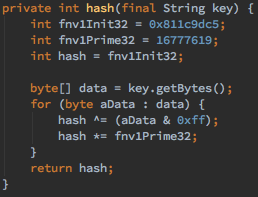
\includegraphics[scale=0.5]{hashfunction}
	\caption{Fonction de hachage FNV1}
\end{center}
\end{figure}

La fonction de hachage FNV1 n'est pas une fonction de hachage parfaite. Une fonction de hachage est dite parfaite si elle n'engendre aucune collision. En effet, nous avons toujours le problème de collision. Pour le résoudre, chaque case ou \textit{bucket} contient une liste chaînée. Si deux clés se retrouvent au même \textit{bucket}, les deux paires clé-valeur seront stockées dans cette liste.

Voici la représentation graphique de notre dictionnaire de données :
\begin{figure}[H]
\begin{center}
	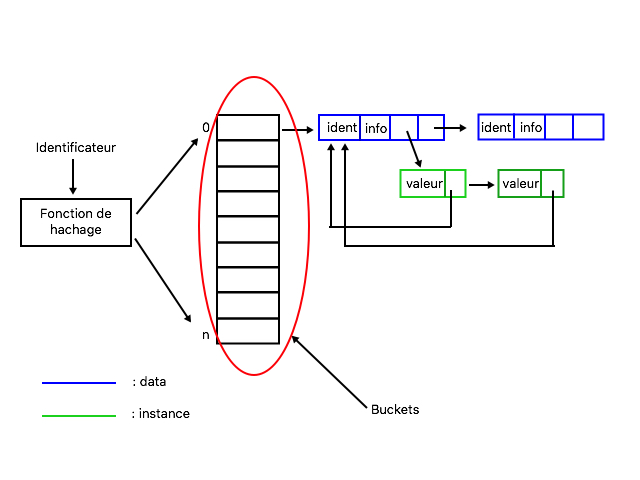
\includegraphics[scale=0.5]{hashmap}
	\caption{Dictionnaire de données}
\end{center}
\end{figure} 

L'image est notre dictionnaire de données. La table de hachage a pour capacité initiale \textbf{n}, c'est-à-dire qu'il contient n \textit{buckets}. Comme mentionné avant, chaque \textit{bucket} contient une liste de data. Data est un nœud de la liste, chaque data contient un identificateur, les informations concernant la variable, le tableau, ou la méthode déclarée. Chaque data possède une liste d'instances. Chaque instance possède une valeur et un pointeur vers son data pour récupérer les information concernant cette instance. 

Notre dictionnaire de données sert à stocker les données déclarées dans un programme Minijaja. Par exemple, lors du déclaration d'une variable de type entier:

\begin{lstlisting}
int test = 3;
\end{lstlisting}

Cette déclaration a pour l'identificateur la chaîne de caractères "test". Pour stocker cette déclaration dans le dictionnaire, on prends l'identificateur et on implémente la fonction de hachage à cet identificateur. Le résultat de cette fonction est un nombre qui indique l'indice du \textit{bucket} dans lequel la donnée sera stockée. Si, par exemple la fonction de hachage transforme la chaîne "test" en un nombre 0, on crée un nœud data, ce nœud a pour l'identificateur "test". La nature de l'objet est \textit{variable} et le type d'objet est \textit{integer}, ces deux informations sont aussi stockées dans le nœud data. Nous ajoutons aussi un nœud instance à la liste d'instances du nœud data, ce nœud instance a pour valeur 3. Nous ajoutons le nœud data à la liste chaînée du \textit{bucket} à l'indice 0.

Notre table de hachage a pour \textit{load factor} 0.75, c'est-à-dire que si le nombre d'éléments atteint 75\% de la capacité initiale, nous augmentons la capacité de la table de hachage. Ceci est fait pour diminuer la taille de la liste chaîne que chaque \textit{bucket} possède pour garder la complexité de la recherche d'un élément dans la table.

L'intérêt de l'utilisation de la table de hachage est la complexité de la recherche d'un élément. Comme les tables ordinaires, la table de hachage permet un accès en O(1) en moyenne. Toutefois, comme plusieurs paires clé-valeur peuvent se trouver dans un même \textit{bucket}, le temps d'accès dans le pire cas est de O(n).
 
 
\subsection{Le tas}
Le tas sert à stocker les données d'un tableau. Lors que l'utilisateur déclare un tableau d'une taille dans le programme Minijaja, les données de ce tableau sont stockées dans le tas. Le tas lui-même est un tableau.

Lors que le tas est initialisé, Le tas est initialisé avec une capacité donnée ou une capacité par défaut. Le capacité par défaut est de 256. Voici le tas après l'initialisation. Supposons que le tas a pour capacité sa capacité par défaut. Le tas possède un bloc libre de taille 256 à l'adresse 0.

\begin{figure}[H]
\begin{center}
	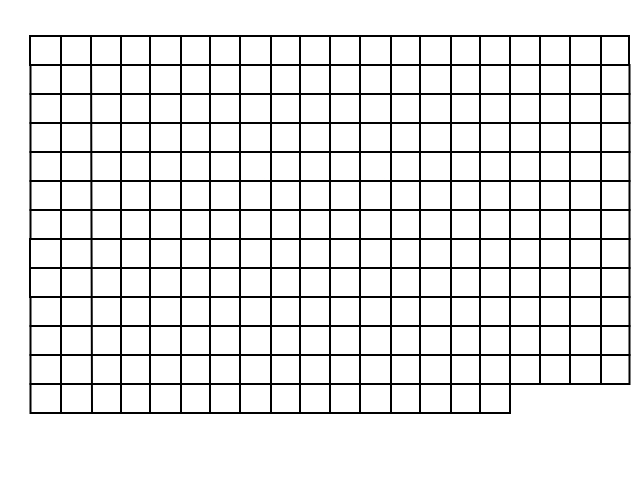
\includegraphics[scale=0.5]{initializetas}
	\caption{Initialisation du tas}
\end{center}
\end{figure} 

Nous avons aussi une table pour mémoriser les adresses des blocs libres dans le tes. Chaque case du tableau contient des adresses des blocs libres dont la taille est de 2 \^{} l'indice de la case dans le tableau. Par exemple, la case 0 contient des adresses des blocs libres de taille 2 \^{} 0 = 1.

Après l'initialisation du tas, la table d'adresses des blocs libres du tas indique qu'il y a un bloc libres de taille 256 à l'adresse 0.

\begin{figure}[H]
\begin{center}
	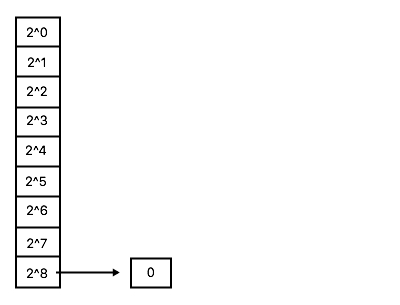
\includegraphics[scale=0.5]{adress}
	\caption{La table d'adresses des blocs libres du tas après l'initialisation du tas}
\end{center}
\end{figure}

Imaginons que l'utilisateur déclare un tableau "t1" de taille 10. Nous parcourons la table d'adresses pour chercher un bloc dont la taille est égale ou supérieure à 10. Nous avons trouvé un bloc de taille 256 à l'adresse 0. Ce bloc est ensuite découpé.

\begin{figure}[H]
\begin{center}
	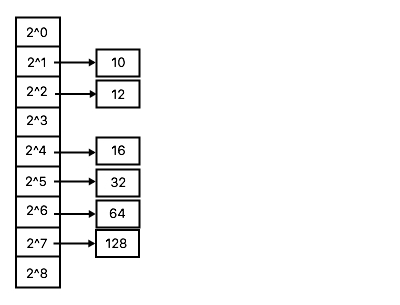
\includegraphics[scale=0.5]{adress2}
	\caption{Le tableau d'adresses des blocs libres du tas après la déclaration d'un tableau de taille 10}
\end{center}
\end{figure}

Nous pouvons regarder qu'il nous reste 6 blocs avec la taille totale de 246. Les éléments du tableau "t1" seront stocké dans le tas dans le bloc de taille 10 situé à l'adresse 0 jusqu'à l'adresse 9.

\begin{figure}[H]
\begin{center}
	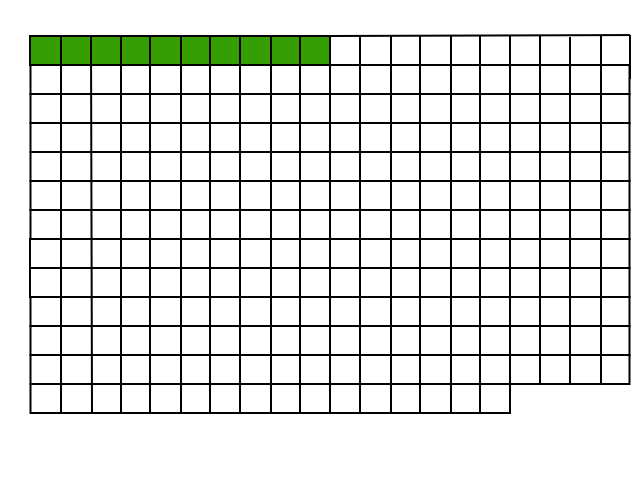
\includegraphics[scale=0.5]{tas2}
	\caption{Le tas après la déclaration du tableau de taille 10}
\end{center}
\end{figure}

Le bloc en vert est le bloc destiné à stocker les éléments du tableau "t1".

Supposons que l'utilisateur déclare ensuite un tableau "t2" de taille 3. Nous parcourons la table d'adresses de blocs libres, nous trouvons un bloc de taille 4 à l'adresse 12, nous découpons ce bloc.

\begin{figure}[H]
\begin{center}
	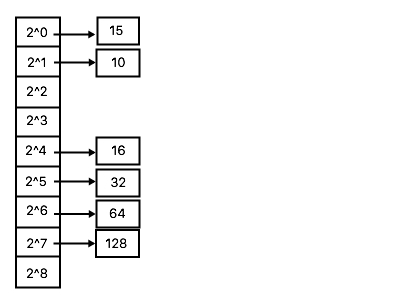
\includegraphics[scale=0.5]{adress3}
	\caption{La table d'adresses des blocs libres du tas après la déclaration d'un tableau de taille 3}
\end{center}
\end{figure}

En effet, les éléments du tableau "t2" seront stockés dans le bloc situé l'adresse 12 jusqu'à l'adresse 14.

\begin{figure}[H]
\begin{center}
	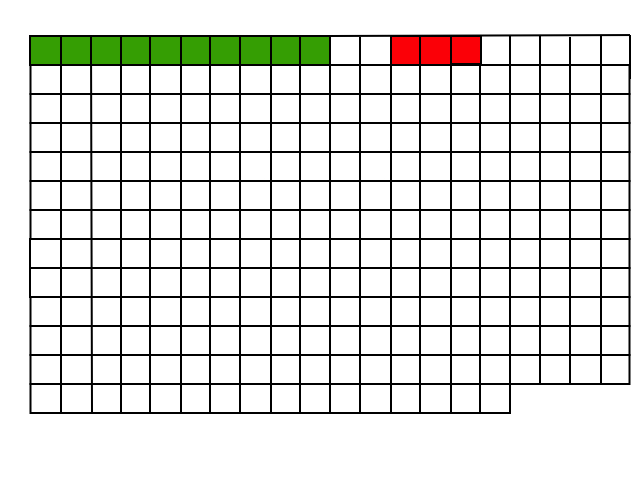
\includegraphics[scale=0.5]{tas3}
	\caption{Le tas après la déclaration du tableau de taille 3}
\end{center}
\end{figure}

Le bloc en rouge est le bloc destiné à stocker les éléments du tableau "t2".

Un problème apparaît. Comme ce que nous pouvons voir, il y a deux espaces libres entre le bloc en vert et le bloc en rouge, c'est le problème de fragmentation. Ces deux espaces risquent d'être perdu. Pour résoudre ce problème, nous faisons en sorte qu'à chaque déclaration du tableau, le bloc destiné à stocker ses données est aligné au plus gauche possible. Nous faisons aussi des fusionnement des blocs qui nécessitent d'être fusionnés.

\begin{figure}[H]
\begin{center}
	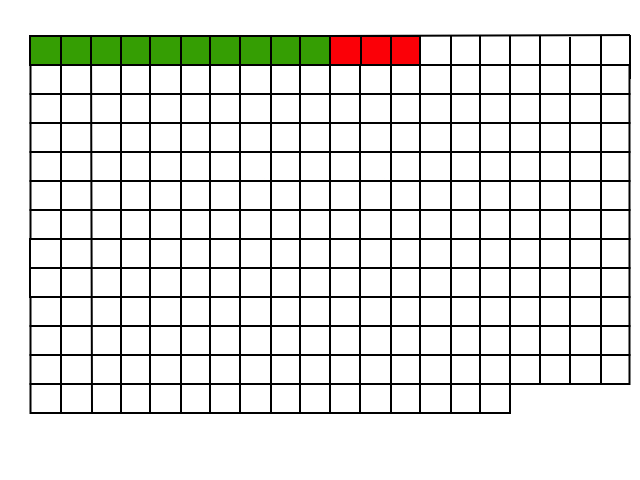
\includegraphics[scale=0.5]{tas4}
	\caption{Le nouveau bloc est aligné au plus gauche possible}
\end{center}
\end{figure}

\begin{figure}[H]
\begin{center}
	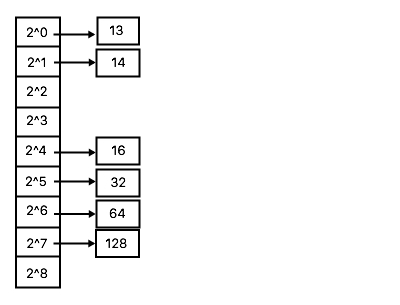
\includegraphics[scale=0.5]{adress4}
	\caption{La table d'adresses des blocs libres après l'alignement du bloc t2 au plus gauche possible}
\end{center}
\end{figure}

La même opération est faite lors de la suppression du bloc du tas. De cette manière, les blocs libres sont toujours regroupés à droite des blocs assignés. Et il n'y a pas de blocs libres situés entre des blocs assignés.

Nous avons aussi une table de symbole pour mémoriser les blocs assignés. Dans notre exemple, la table de symbole est comme ci-dessus:

\begin{figure}[H]
\begin{center}
	\begin{tabular}{ |c|c|c|c| }
	\hline
	Identificateur & adresse & taille & références \\
	\hline	
	1 & 0 & 10 & 1 \\
	\hline
	2 & 10 & 3 & 1 \\
	\hline
	\end{tabular}
	\caption{La table de symbole du tas}
\end{center}
\end{figure}

L'identificateur du bloc est la clé de cette table. Pour chaque clé, nous avons l'adresse du bloc, la taille du bloc, et aussi le nombre de références pour ce bloc. 


\subsection{La pile}
La pile sert à stocker les instances des variables, des tableaux, et des méthodes déclarées dans le programme Minijaja. Par exemple, lors de la déclaration des deux variables de type entier :

\begin{lstlisting}
int i = 3;
int j = 4;
\end{lstlisting}

Lors de la déclaration de ces deux variables, nous ajoutons à la table de hachage deux nœuds data, et nous ajoutons aussi deux instances à la pile. 

\begin{center}
	\textless i,INTEGER,VARIABLE,3\textgreater \\
	\textless j,INTEGER,VARIABLE,4\textgreater
\end{center}

Toutes les opérations se baseront sur la pile. Dans le cas où l'instance est un tableau, sa valeur est l'identificateur du bloc contenant les éléments du tableau dans le tas. Et dans le cas où l'instance est une méthode, sa valeur est le nœud AST de la méthode.

\subsection{La Mémoire}
La mémoire contient trois éléments : le dictionnaire de données, le tas, et la pile. Lors de la déclaration d'une donnée, l'identificateur et les informations de la donnée sont stocké dans le dictionnaire de données, la valeur de la donnée est stockée dans la pile. Dans le cas de la déclaration d'une tableau, ses éléments sont stockés dans le tas.

Les opérations qui peuvent être effectuées par la mémoire sont :

\begin{figure}[H]
\begin{center}
	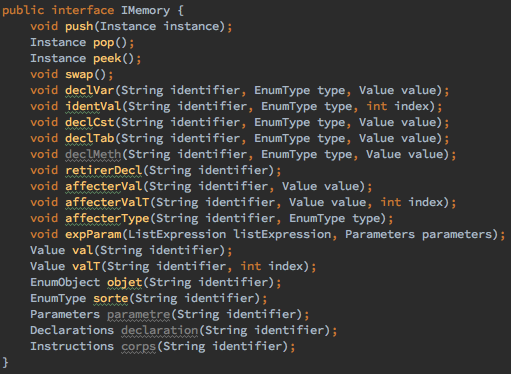
\includegraphics[scale=0.5]{memoire}
	\caption{Les opérations de la mémoire}
\end{center}
\end{figure}

\section{Traitement des erreurs}
Les erreurs peuvent apparaître lors des opérations dans la mémoire. Lors que une erreur est produite, une exception est levée. Par exemple, dans le cas où l'utilisateur essaie d'affecter une valeur à une variable dans la pile, mais la pile est vide. Une exception du type NullStackException est levée.

\begin{figure}[H]
\begin{center}
	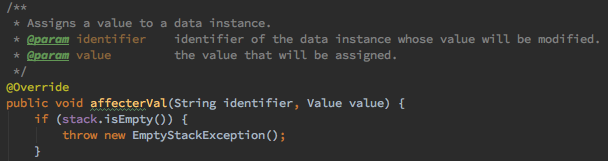
\includegraphics[scale=0.5]{affecterval}
	\caption{L'affectation de la variable dans le cas où la pile est vide}
\end{center}
\end{figure}

Il existe plusieurs autres exceptions dans la mémoire. Ces exceptions sont aussi utile pour le contrôle de type.

\section{Choix de test}
Nous effectuons des tests fonctionnels pour chaque fonctionnalité de la mémoire et ses composants. Par exemple, la table de hachage est un composant de la mémoire, nous faisons des tests pour s'assurer que la table de hachage fonctionne correctement. Nous avons un test qui s'assure que la table de hachage augmente sa capacité si le nombre des éléments contenus dans la table de hachage atteint 75\% de sa capacité, nous avons aussi un test qui s'assure que lors de l'insertion d'une valeur avec une clé qui existe déjà dans la table de hachage, l'ancienne valeur est supprimée et remplacée par la nouvelle valeur. Voici la capture de ce test.

\begin{figure}[H]
\begin{center}
	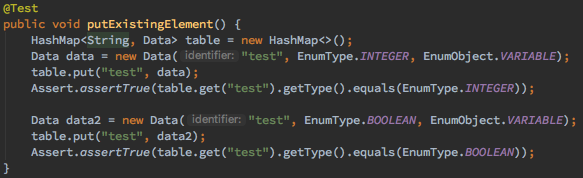
\includegraphics[scale=0.5]{testexisting}
	\caption{Un exemple du test fonctionnel de la table de hachage}
\end{center}
\end{figure}

Nous pouvons remarquer aussi que pour chaque test fonctionnel, nous déclarons de nouveau l'élément que nous testons. Dans l'image ci-dessus, nous déclarons la table de hachage au début du test. Nous n'utilisons pas une seule table de hachage pour tous les tests. Nous avons décidé de faire ce choix pour que chaque test ne dépend pas des autres test, autrement dit, chaque test est indépendant et peut être exécuté individuellement. 

Cependant, dans certains cas, nous avons besoin de tester une fonctionnalité avant de tester une autre fonctionnalité parce que la deuxième fonctionnalité a besoin d'appeler la première fonctionnalité. Par exemple, pour tester la méthode d'affectation d'une valeur à une variable dans la pile, nous avons besoin d'utiliser la méthode de la déclaration de la variable. C'est la raison pour laquelle nous devons être surs que la méthode de la déclaration de la variable fonctionne normalement avant de pouvoir l'utiliser. Autrement dit, nous avons besoin de tester la déclaration de la variable avant l'affectation de la valeur à une variable.

\begin{figure}[H]
\begin{center}
	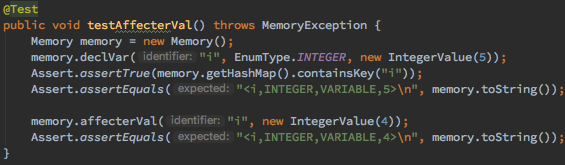
\includegraphics[scale=0.5]{testaffectation}
	\caption{Le test de l'affectation d'une valeur à une variable}
\end{center}
\end{figure}

\end{document}